\documentclass[10pt, letterpaper]{article} % Letter paper gives 8.5 x 11 paper.

% Preamble (the section between \documentclass and \begin{document}) is where we put the packages.

% Packages

% \usepackage{fullpage} % Makes document have 1 inch margins everywhere.
\usepackage[margin=1in]{geometry} % Has same effect as above line.
% \usepackage[top=1in, bottom=1in, left=1in, right=1in]{geometry} % Same as above line

% \usepackage{amsfonts} % Allows us to use some specialized math notation (ie R).
\usepackage{amsfonts, amssymb, amsmath}
\usepackage{tikz, pgfplots} % For calculator command.
\usepackage{graphicx} % Allows us to insert images.
\usepackage{float} % Useful for placing images/tables.

% Marcos
% \def % def is to define a new command
\def\eq1{y = \dfrac{x}{3x^2+x+1}} % Whenever we type \eq1, this equation will be produced.

\newcommand{\set}[1] {\setlength\itemsep{#1}} % Adds separation between list items.

\newcommand\calculator{\tikz{
		\node (c) [inner sep=0pt, draw, fill=black, anchor=south west]{\phantom{N}};
		\begin{scope}[x=(c.south east),y=(c.north west)]    \fill[white] (.1,.7) rectangle (.9,.9);    
		\foreach \x in {.1, .33, .55, .79}{    
		\foreach \y in {.1, .24, .38, .53}{    
		\fill[white] (\x,\y) rectangle +(.11,.07);}} 
		\end{scope} }}
		\def\calcicon#1{\noindent#1 \calculator\ }

\begin{document}

\textbf{Critical Thinking Questions}

% Inserting image.
% 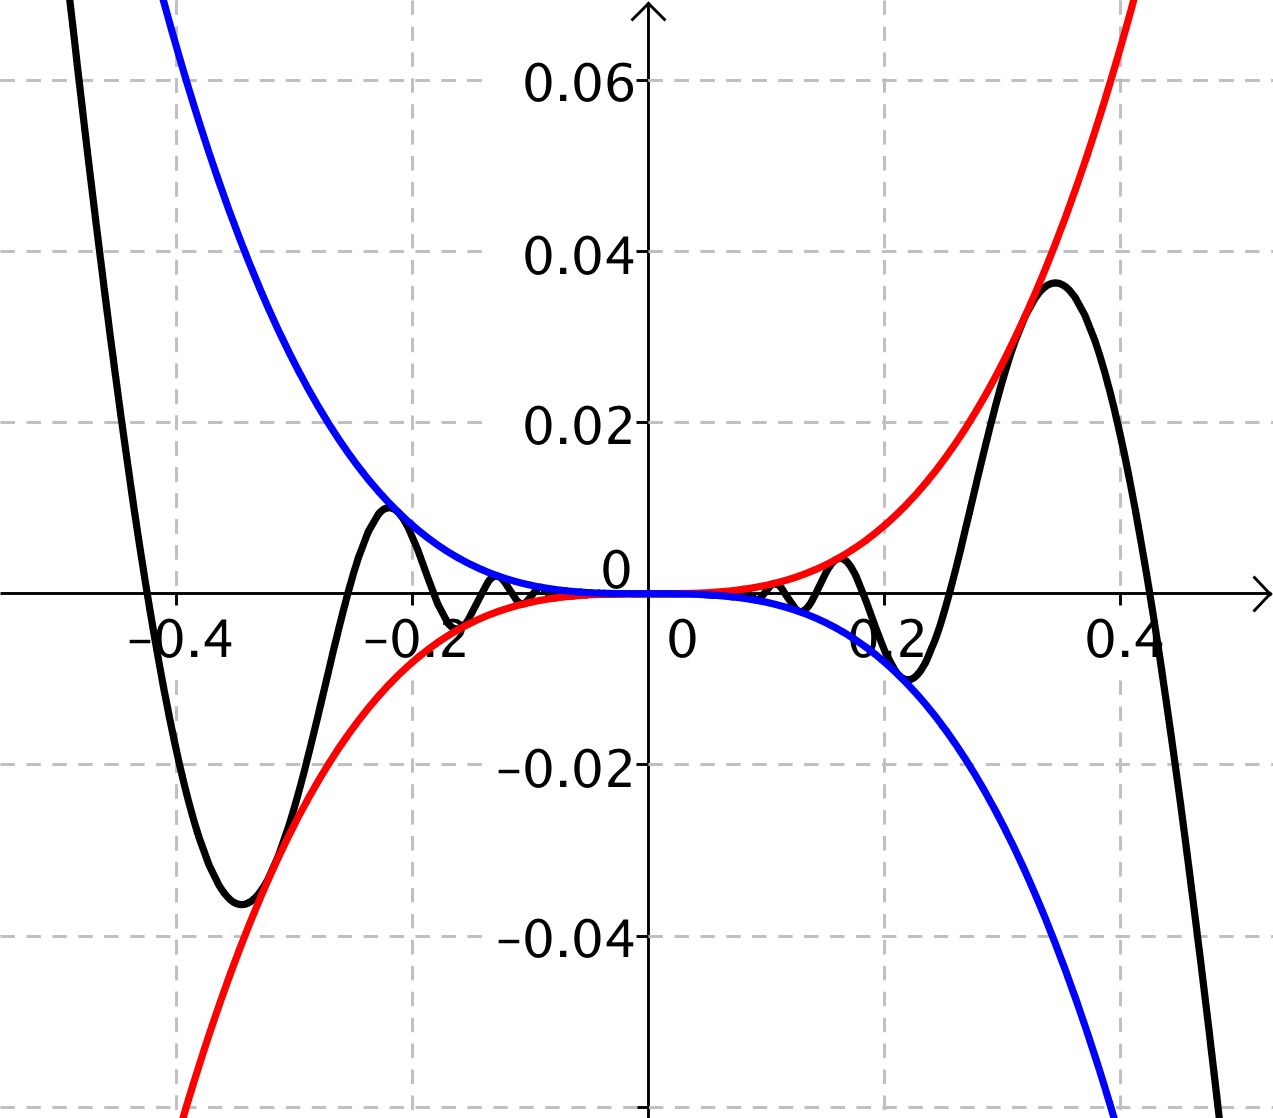
\includegraphics[scale=0.6]{limit.png} % Scaling size
% 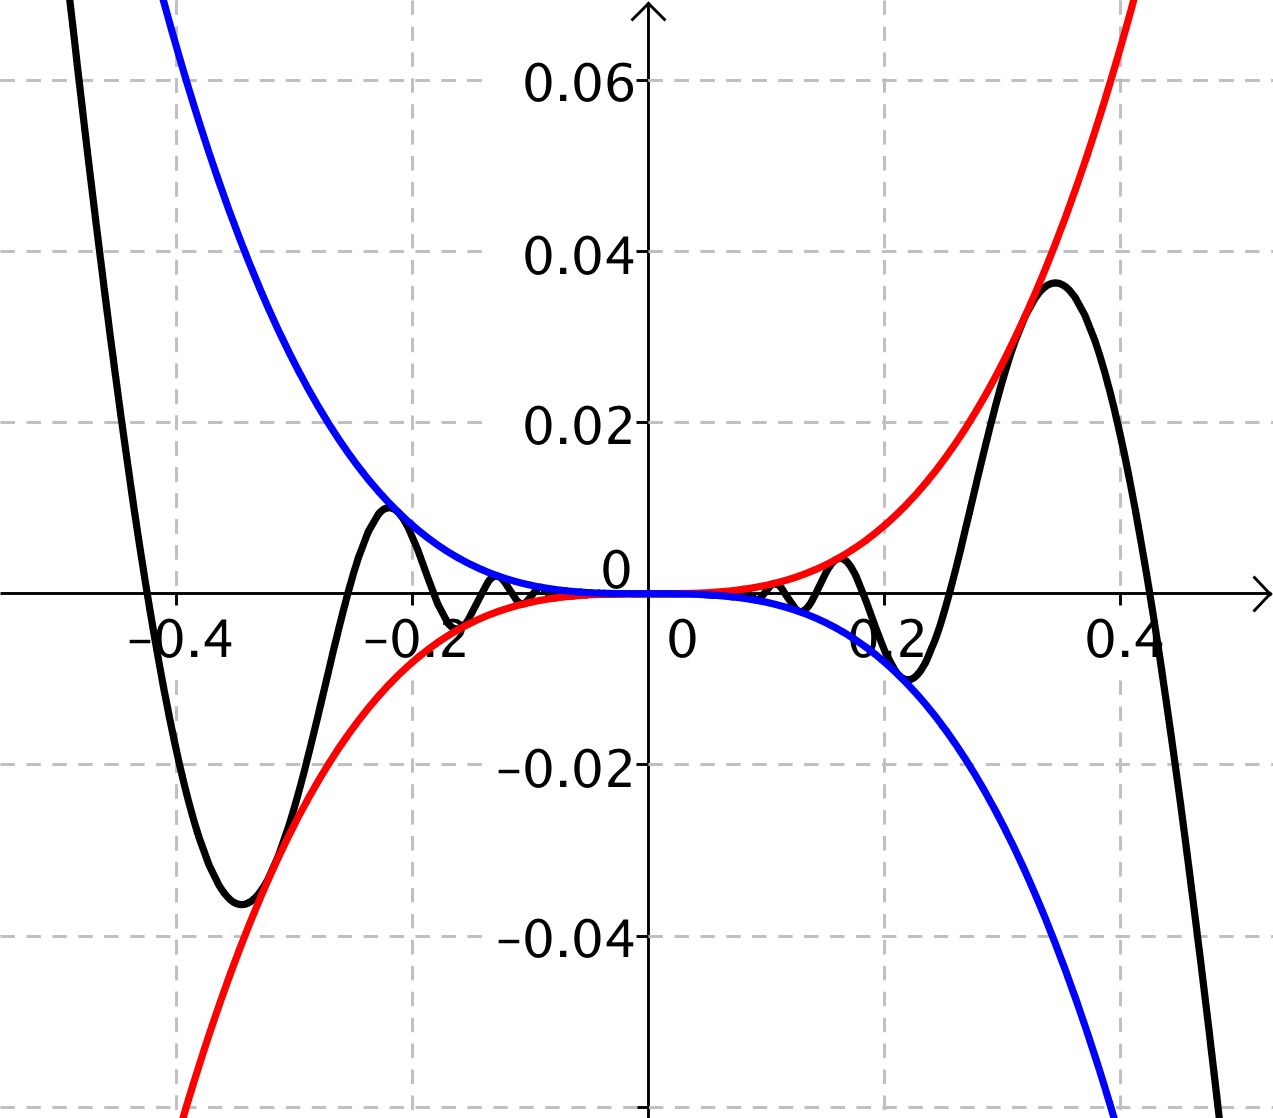
\includegraphics[scale=0.5\textwidth]{limit.png} % Scaling size to half of the textwidth.
\begin{center} % Center image.
	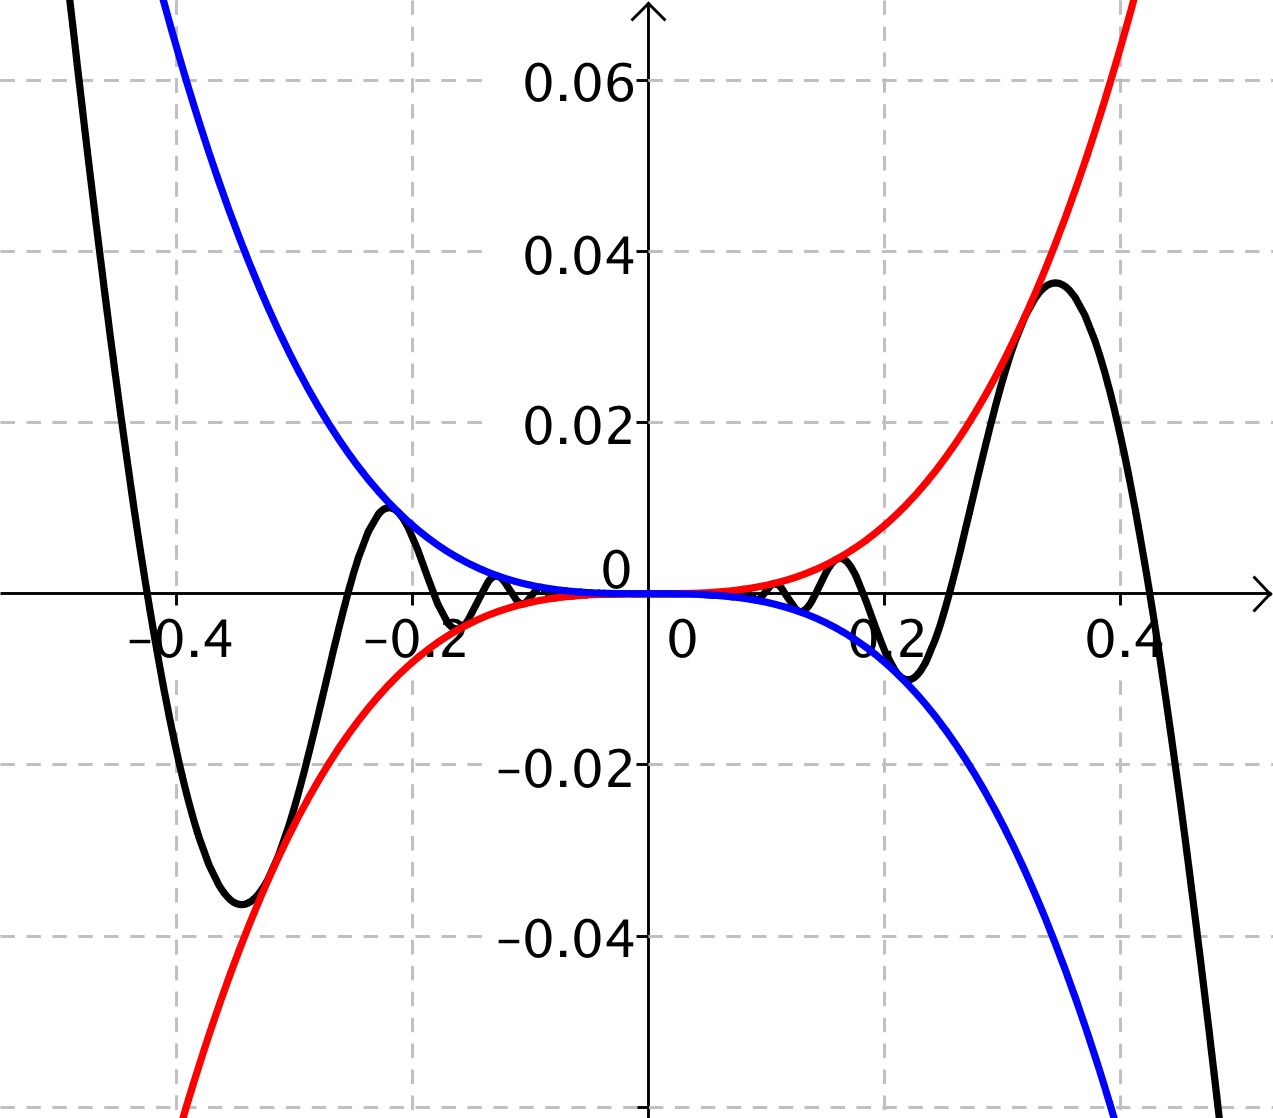
\includegraphics[width=3.5in]{limit.png} % Typically only change width or height, otherwise photo will deform.	
\end{center}

\begin{figure}[H] % h = here, b = bottom, t = top. H works always, but need to use float package.
	\centering % Centers everything in this env.
	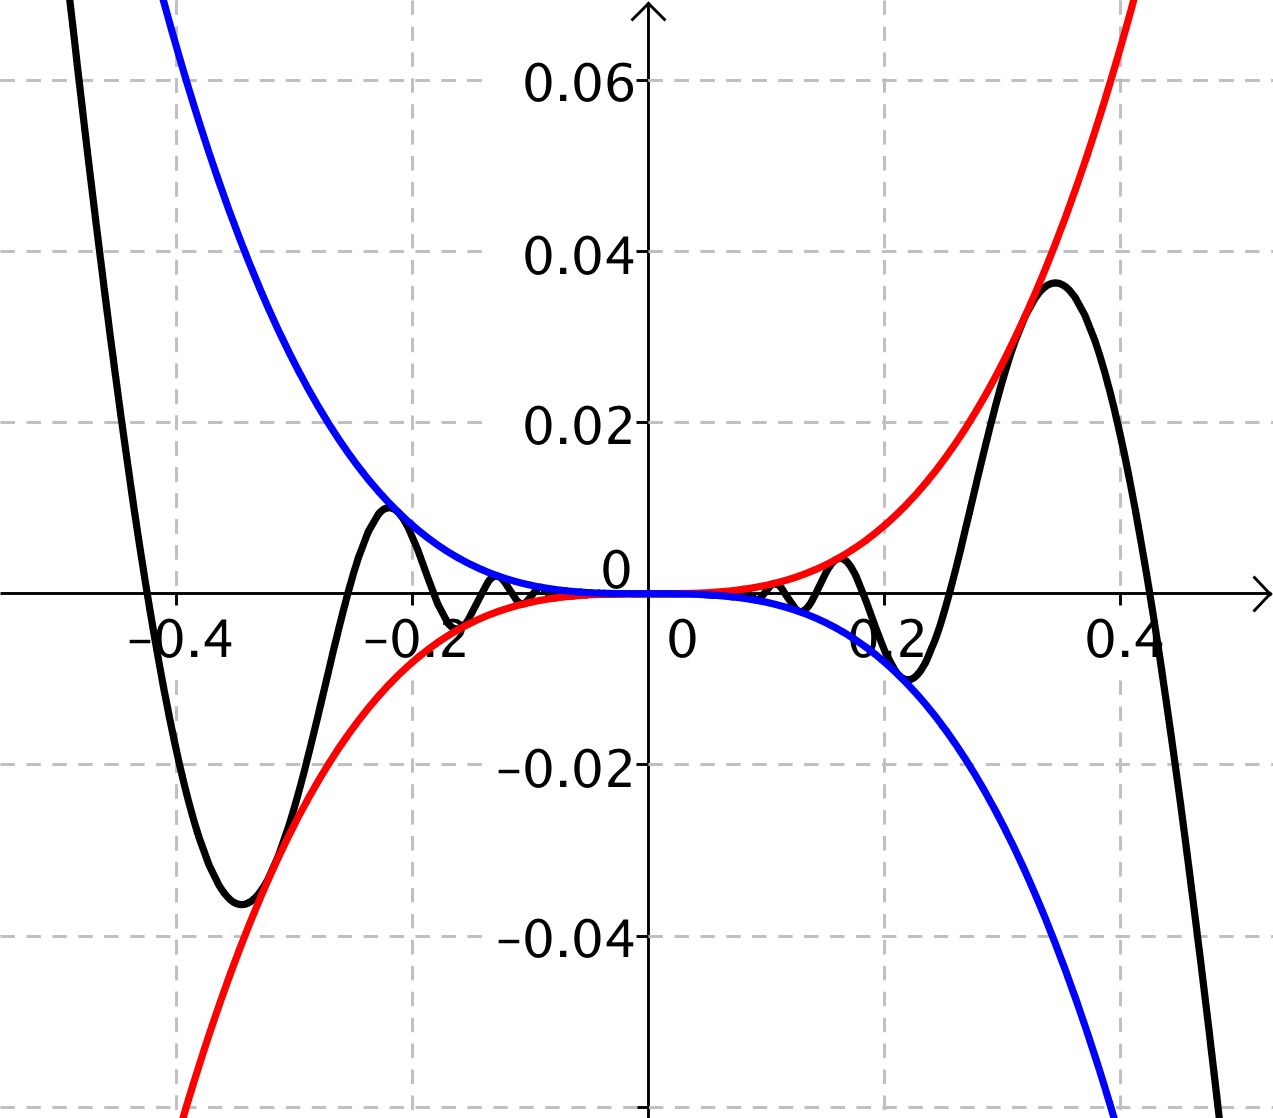
\includegraphics[width=3.5in]{limit.png} % Typically only change width or height, otherwise photo will deform.	
	\caption{This Squeeze Theorem}
\end{figure}


\begin{enumerate}
	\set{1.2pt}
	\item \calculator\ Let's examine the function $ \eq1 $.
	\item This is the symbol for the set of all real numbers: $\mathbb{R}$.
	\item This is the symbol for the set of all integers: $\mathbb{Z}$.
	\item This is the symbol for the set of all rationals: $\mathbb{Q}$.
	\item Is it possible for a sequence to converge to two different numbers? If so, give an example. If not, explain why not.
	\item Explain how to use partial sums to determine if a series converges or diverges. Give an example.
	\item Explain why $ \int\limits_{1}^{\infty} f(x)\, dx $ and $ \sum\limits_{n=1}^{\infty} a_n $ need not converge to the same value, even if they are both convergent.
	\item In your own words, explain the Alternating Series Remainder Theorem.
	\item Explain the difference between absolute and conditional convergence. Give an example of each.
	\item The Ratio Test is inconclusive if $ \displaystyle{\lim\limits_{n \to \infty} \left| \frac{a_{n+1}}{a_n} \right| =1} $. Give an example of one convergent series and one divergent series for which $ \displaystyle{\lim\limits_{n \to \infty} \left| \frac{a_{n+1}}{a_n} \right| =1} $. Explain how you determined your examples.
\end{enumerate}

\end{document}



